\documentclass{article}
\usepackage{polski}
\usepackage[utf8]{inputenc}

\usepackage{graphicx}
\graphicspath{ {../img/} }

\usepackage{graphicx}
\usepackage{enumitem}
\usepackage{amsmath}

\title{F5 - Badanie dwójłomności CdS i CdSe}
\author{Jolanta Niedźwiecka}
% \date{18 sierpnia 2021}
%-----------------------------------------------------------
\begin{document}
    \maketitle

% \begin{abstract}
%     Lorem ipsum
% \end{abstract}

% \section{Teoria}

\section{Czułość}

    W tej części doświadczenia zbadano czułość detektorów w zależności od energii padającego światła. Jak widać, zakres czułości detektora 1 przypada na 1-2,4 eV, natomiast detektor 2 jest czuły w zakresie 0,5-1,4 eV.

    \begin{figure}[h]
        \centering
        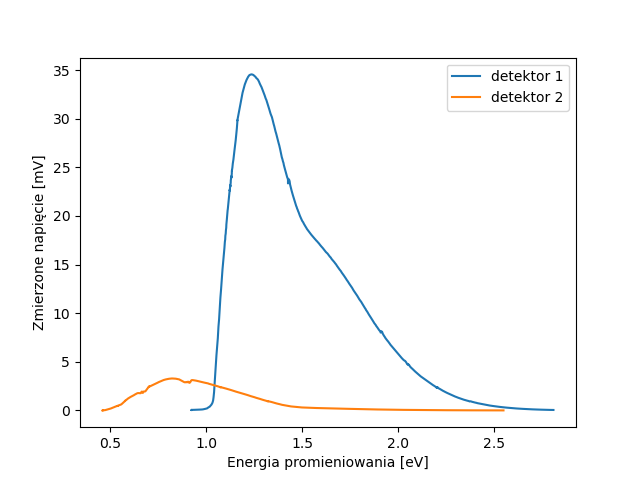
\includegraphics[width=0.9\textwidth]{sensitivity.png}
        \caption{Porównanie zakresów czułości dwóch detektorów}
    \end{figure}

\section{Dobroć układu polaryzatorów}

    \begin{equation}
        D(\hbar\omega)=
        \frac{I_\parallel(\hbar\omega)-I_\perp(\hbar\omega)}
        {I_\parallel(\hbar\omega)+I_\perp(\hbar\omega)}
    \end{equation}
    $I_\parallel$ - natężenie światła po przejściu przez układ polaryzatorów ustawionych równolegle względem siebie; $I_\perp$ - natężenie światła po przejściu przez układ polaryzatorów ustawionych prostopadle względem siebie.

    Dobroć jest obliczana dla dwóch układów polaryzatorów (nowego i starego) i dla dwóch detektorów - w sumie 4 wyniki.

\end{document}
